%
% gleichverteilung.tex -- Abschnitt über Gleichverteilung in Kapitel 5
%
% (c) 2015 Prof Dr Andreas Mueller, Hochschule Rapperswil
%
\subsection{Gleichverteilung} \label{section-gleichverteilung-stetig}
\begin{table}
\renewcommand{\arraystretch}{1.5}
\begin{center}
\begin{tabular}{|l|l|}
\hline
Name&Gleichverteilung\\
\hline
Dichtefunktion&
\begin{minipage}{3.7in}
\vskip5pt
$\displaystyle
\begin{cases}
\displaystyle \frac1{b-a}&\qquad a\le x\le b\\
0&\qquad\text{sonst}
\end{cases}
$
\end{minipage}
\\[8pt]
Verteilungsfunktion&
\begin{minipage}{3.7in}
\vskip5pt
$\displaystyle
\begin{cases}0&\qquad x\le a\\
\displaystyle \frac{x-a}{b-a}&\qquad x \le a \le b\\
1&\qquad x>b\end{cases}
$
\end{minipage}
\\[8pt]
Erwartungswert&
\begin{minipage}{3.7in}
\vskip3pt
$\displaystyle \frac{a+b}2$
\end{minipage}
\\[8pt]
Varianz&
\begin{minipage}{3.7in}
\vskip3pt
$\displaystyle \frac{(b-a)^2}{12}$
\end{minipage}
\\[8pt]
Median&
\begin{minipage}{3.7in}
\vskip3pt
$\displaystyle \frac{a+b}{2}$
\end{minipage}
\\[8pt]
$P(|X-E(X)|>\varepsilon)$&
\begin{minipage}{3.7in}
\vskip3pt
$\displaystyle 1-\frac{2\varepsilon}{b-a}$ f"ur $\varepsilon<\displaystyle \frac{b-a}2$
\end{minipage}
\\[10pt]
\hline
Anwendungen&\begin{minipage}{3.7in}%
\strut
$\bullet$ Verteilung von Zufallszahlen
\strut
\end{minipage}\\
\hline
\end{tabular}
\end{center}
\caption{Datenblatt der Gleichverteilung\label{datenblatt:gleichverteilung}}
\end{table}

\begin{figure}
\begin{center}
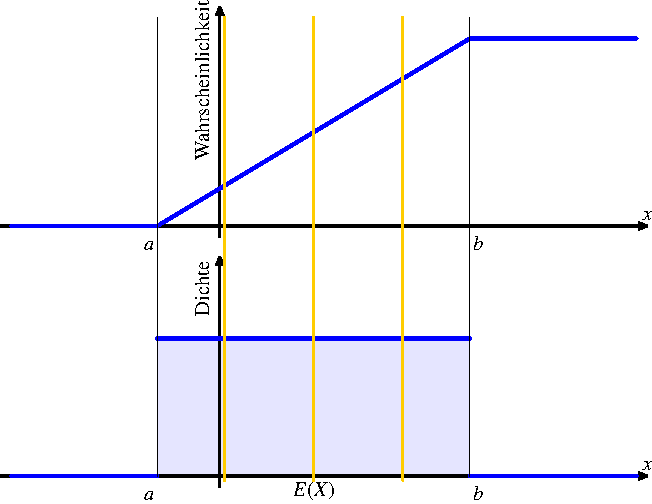
\includegraphics[width=0.8\hsize]{images/verteilungsfunktion-7}
\end{center}
\caption{Verteilungsfunktion (oben) und Wahrscheinlichkeitsdichte (unten)
der Gleichverteilung\label{bild-gleichverteilung}}
\end{figure}
\begin{figure}
\begin{center}
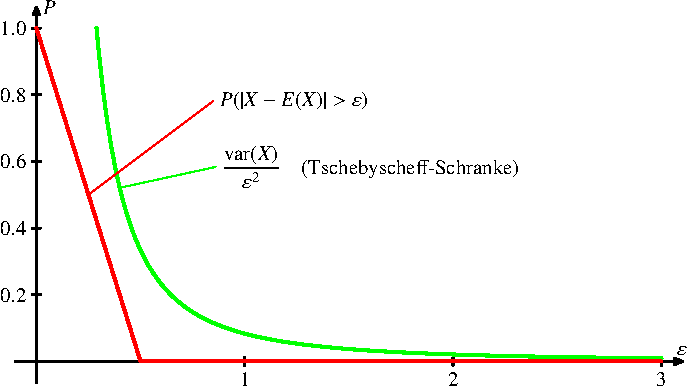
\includegraphics{images/gl-1.pdf}
\end{center}
\caption{Wahrscheinlichkeit einer Abweichung vom Mittelwert einer
in $[0,1]$ gleichverteilten Zufallsvariable (rot) im Vergleich mit
der oberen Schranke aus dem Satz von Tschebyscheff (gr"un)
\label{bild-gleichverteilung-wahrscheinlichkeit}} % changed
\end{figure}
Gleichverteilung der Werte einer Zufallsvariablen liegt vor, wenn
die Wahrscheinlichkeit, dass ein Wert in ein bestimmtes Intervall
f"allt, der L"ange des Intervalles proportional ist. Dies bedeutet,
dass die Verteilungsfunktion $F$ konstante Steigung hat. Da $0\le F(x)\le 1$
gelten muss, ist dies nur innerhalb eines Intervalls $[a,b]$ m"oglich.
\begin{definition}Die Zufallsvariable $X$ heisst auf dem Intervall
$[a,b]$ gleichverteilt, wenn sie die Verteilungsfunktion
\[
F(x)=\begin{cases}
0&\qquad x< a\\
\displaystyle \frac{x-a}{b-a}&\qquad x\in[a,b]\\
1&\qquad x> b
\end{cases}
\]
mit der Wahrscheinlichkeitsdichte
\[
\varphi(x)=\begin{cases}
0&\qquad x< a\\
\displaystyle \frac1{b-a}&\qquad x\in[a,b]\\
0&\qquad x> b
\end{cases}
\]
hat.
\end{definition}

\subsubsection{Erwartungswert und Varianz}
\begin{satz}Sei $X$ eine in $[a,b]$ gleichverteilte Zufallsvariable,
dann gilt
\begin{align*}
E(X)&=\frac{a+b}2\\
\operatorname{var}(X)&=\frac{(b-a)^2}{12}
\end{align*}
\end{satz}
\begin{proof}[Beweis]
Mit Hilfe der Dichtefunktion berechnet man den Erwartungswert
\begin{align*}
E(X)&=\int_{-\infty}^\infty \varphi(x)x\,dx=\int_a^b\frac{x}{b-a}\,dx\\
&=\frac1{b-a}\left[\frac12x^2\right]_a^b=\frac{b^2-a^2}{2(b-a)}=\frac{a+b}2
\end{align*}
und die Varianz
\begin{align*}
E(X^2)=&\int_{-\infty}^\infty x^2\varphi(x)\,dx=\frac1{b-a}\int_a^bx^2\,dx\\
&=\frac1{b-a}\left[\frac{x^3}3\right]_a^b=\frac{b^3-a^3}{3(b-a)}=\frac{a^2+ab+b^2}3\\
\operatorname{var}(X)&=\frac{a^2+ab+b^2}3-\frac{(b+a)^2}4\\
&=\frac{4a^2+4ab+4b^2-3b^2-6ab-3a^2}{12}\\
&=\frac{a^2-2ab+b^2}{12}=\frac13\left(\frac{b-a}2\right)^2\\
\sqrt{\operatorname{var}(X)}&=\frac1{\sqrt{3}}\cdot\frac{b-a}2\simeq 0.57\cdot\frac{b-a}2.
\end{align*}

\end{proof}

\subsubsection{Wahrscheinlichkeit einer grossen Abweichung}
{\small
F"ur $\varepsilon>\frac{b-a}2$ ist die Wahrscheinlichkeit
$P(|X-\mu|>\varepsilon)$
einer Abweichung vom Erwartungswert $\mu=E(X)$ nat"urlich $0$,
aber f"ur kleinere $\varepsilon$ ergibt sich
\begin{align*}
P(|X-\mu|>\varepsilon)
&=1-\int_{\mu-\varepsilon}^{\mu+\varepsilon}\varphi(x)\,dx
=1-\int_{\mu-\varepsilon}^{\mu+\varepsilon}\frac{1}{b-a}\,dx\\
&=1-\frac1{b-a}\left[x\right]_{\mu-\varepsilon}^{\mu+\varepsilon}=1-\frac{2\varepsilon}{b-a}
\end{align*}
}
